
%% bare_conf.tex
%% V1.4
%% 2012/12/27
%% by Michael Shell
%% See:
%% http://www.michaelshell.org/
%% for current contact information.
%%
%% This is a skeleton file demonstrating the use of IEEEtran.cls
%% (requires IEEEtran.cls version 1.8 or later) with an IEEE conference paper.
%%
%% Support sites:
%% http://www.michaelshell.org/tex/ieeetran/
%% http://www.ctan.org/tex-archive/macros/latex/contrib/IEEEtran/
%% and
%% http://www.ieee.org/

%%*************************************************************************
%% Legal Notice:
%% This code is offered as-is without any warranty either expressed or
%% implied; without even the implied warranty of MERCHANTABILITY or
%% FITNESS FOR A PARTICULAR PURPOSE! 
%% User assumes all risk.
%% In no event shall IEEE or any contributor to this code be liable for
%% any damages or losses, including, but not limited to, incidental,
%% consequential, or any other damages, resulting from the use or misuse
%% of any information contained here.
%%
%% All comments are the opinions of their respective authors and are not
%% necessarily endorsed by the IEEE.
%%
%% This work is distributed under the LaTeX Project Public License (LPPL)
%% ( http://www.latex-project.org/ ) version 1.3, and may be freely used,
%% distributed and modified. A copy of the LPPL, version 1.3, is included
%% in the base LaTeX documentation of all distributions of LaTeX released
%% 2003/12/01 or later.
%% Retain all contribution notices and credits.
%% ** Modified files should be clearly indicated as such, including  **
%% ** renaming them and changing author support contact information. **
%%
%% File list of work: IEEEtran.cls, IEEEtran_HOWTO.pdf, bare_adv.tex,
%%                    bare_conf.tex, bare_jrnl.tex, bare_jrnl_compsoc.tex,
%%                    bare_jrnl_transmag.tex
%%*************************************************************************

% *** Authors should verify (and, if needed, correct) their LaTeX system  ***
% *** with the testflow diagnostic prior to trusting their LaTeX platform ***
% *** with production work. IEEE's font choices can trigger bugs that do  ***
% *** not appear when using other class files.                            ***
% The testflow support page is at:
% http://www.michaelshell.org/tex/testflow/



% Note that the a4paper option is mainly intended so that authors in
% countries using A4 can easily print to A4 and see how their papers will
% look in print - the typesetting of the document will not typically be
% affected with changes in paper size (but the bottom and side margins will).
% Use the testflow package mentioned above to verify correct handling of
% both paper sizes by the user's LaTeX system.
%
% Also note that the "draftcls" or "draftclsnofoot", not "draft", option
% should be used if it is desired that the figures are to be displayed in
% draft mode.
%
\documentclass[conference]{IEEEtran}
% Add the compsoc option for Computer Society conferences.
%
% If IEEEtran.cls has not been installed into the LaTeX system files,
% manually specify the path to it like:
% \documentclass[conference]{../sty/IEEEtran}





% Some very useful LaTeX packages include:
% (uncomment the ones you want to load)


% *** MISC UTILITY PACKAGES ***
%
%\usepackage{ifpdf}
% Heiko Oberdiek's ifpdf.sty is very useful if you need conditional
% compilation based on whether the output is pdf or dvi.
% usage:
% \ifpdf
%   % pdf code
% \else
%   % dvi code
% \fi
% The latest version of ifpdf.sty can be obtained from:
% http://www.ctan.org/tex-archive/macros/latex/contrib/oberdiek/
% Also, note that IEEEtran.cls V1.7 and later provides a builtin
% \ifCLASSINFOpdf conditional that works the same way.
% When switching from latex to pdflatex and vice-versa, the compiler may
% have to be run twice to clear warning/error messages.






% *** CITATION PACKAGES ***
%
\usepackage{cite}
% cite.sty was written by Donald Arseneau
% V1.6 and later of IEEEtran pre-defines the format of the cite.sty package
% \cite{} output to follow that of IEEE. Loading the cite package will
% result in citation numbers being automatically sorted and properly
% "compressed/ranged". e.g., [1], [9], [2], [7], [5], [6] without using
% cite.sty will become [1], [2], [5]--[7], [9] using cite.sty. cite.sty's
% \cite will automatically add leading space, if needed. Use cite.sty's
% noadjust option (cite.sty V3.8 and later) if you want to turn this off
% such as if a citation ever needs to be enclosed in parenthesis.
% cite.sty is already installed on most LaTeX systems. Be sure and use
% version 4.0 (2003-05-27) and later if using hyperref.sty. cite.sty does
% not currently provide for hyperlinked citations.
% The latest version can be obtained at:
% http://www.ctan.org/tex-archive/macros/latex/contrib/cite/
% The documentation is contained in the cite.sty file itself.






% *** GRAPHICS RELATED PACKAGES ***
%
\ifCLASSINFOpdf
   \usepackage[pdftex]{graphicx}
  % declare the path(s) where your graphic files are
  % \graphicspath{{../pdf/}{../jpeg/}}
  % and their extensions so you won't have to specify these with
  % every instance of \includegraphics
  \DeclareGraphicsExtensions{.pdf,.jpeg,.png}
\else
  % or other class option (dvipsone, dvipdf, if not using dvips). graphicx
  % will default to the driver specified in the system graphics.cfg if no
  % driver is specified.
  % \usepackage[dvips]{graphicx}
  % declare the path(s) where your graphic files are
  % \graphicspath{{../eps/}}
  % and their extensions so you won't have to specify these with
  % every instance of \includegraphics
  % \DeclareGraphicsExtensions{.eps}
\fi
% graphicx was written by David Carlisle and Sebastian Rahtz. It is
% required if you want graphics, photos, etc. graphicx.sty is already
% installed on most LaTeX systems. The latest version and documentation
% can be obtained at: 
% http://www.ctan.org/tex-archive/macros/latex/required/graphics/
% Another good source of documentation is "Using Imported Graphics in
% LaTeX2e" by Keith Reckdahl which can be found at:
% http://www.ctan.org/tex-archive/info/epslatex/
%
% latex, and pdflatex in dvi mode, support graphics in encapsulated
% postscript (.eps) format. pdflatex in pdf mode supports graphics
% in .pdf, .jpeg, .png and .mps (metapost) formats. Users should ensure
% that all non-photo figures use a vector format (.eps, .pdf, .mps) and
% not a bitmapped formats (.jpeg, .png). IEEE frowns on bitmapped formats
% which can result in "jaggedy"/blurry rendering of lines and letters as
% well as large increases in file sizes.
%
% You can find documentation about the pdfTeX application at:
% http://www.tug.org/applications/pdftex





% *** MATH PACKAGES ***
%
\usepackage[cmex10]{amsmath}
% A popular package from the American Mathematical Society that provides
% many useful and powerful commands for dealing with mathematics. If using
% it, be sure to load this package with the cmex10 option to ensure that
% only type 1 fonts will utilized at all point sizes. Without this option,
% it is possible that some math symbols, particularly those within
% footnotes, will be rendered in bitmap form which will result in a
% document that can not be IEEE Xplore compliant!
%
% Also, note that the amsmath package sets \interdisplaylinepenalty to 10000
% thus preventing page breaks from occurring within multiline equations. Use:
%\interdisplaylinepenalty=2500
% after loading amsmath to restore such page breaks as IEEEtran.cls normally
% does. amsmath.sty is already installed on most LaTeX systems. The latest
% version and documentation can be obtained at:
% http://www.ctan.org/tex-archive/macros/latex/required/amslatex/math/





% *** SPECIALIZED LIST PACKAGES ***
%
%\usepackage{algorithmic}
\usepackage{algorithm}
\usepackage{algpseudocode}

%\usepackage{algpseudocode}
% algorithmic.sty was written by Peter Williams and Rogerio Brito.
% This package provides an algorithmic environment fo describing algorithms.
% You can use the algorithmic environment in-text or within a figure
% environment to provide for a floating algorithm. Do NOT use the algorithm
% floating environment provided by algorithm.sty (by the same authors) or
% algorithm2e.sty (by Christophe Fiorio) as IEEE does not use dedicated
% algorithm float types and packages that provide these will not provide
% correct IEEE style captions. The latest version and documentation of
% algorithmic.sty can be obtained at:
% http://www.ctan.org/tex-archive/macros/latex/contrib/algorithms/
% There is also a support site at:
% http://algorithms.berlios.de/index.html
% Also of interest may be the (relatively newer and more customizable)
% algorithmicx.sty package by Szasz Janos:
% http://www.ctan.org/tex-archive/macros/latex/contrib/algorithmicx/




% *** ALIGNMENT PACKAGES ***
%
\usepackage{array}
% Frank Mittelbach's and David Carlisle's array.sty patches and improves
% the standard LaTeX2e array and tabular environments to provide better
% appearance and additional user controls. As the default LaTeX2e table
% generation code is lacking to the point of almost being broken with
% respect to the quality of the end results, all users are strongly
% advised to use an enhanced (at the very least that provided by array.sty)
% set of table tools. array.sty is already installed on most systems. The
% latest version and documentation can be obtained at:
% http://www.ctan.org/tex-archive/macros/latex/required/tools/


% IEEEtran contains the IEEEeqnarray family of commands that can be used to
% generate multiline equations as well as matrices, tables, etc., of high
% quality.




% *** SUBFIGURE PACKAGES ***
\ifCLASSOPTIONcompsoc
  \usepackage[caption=false,font=normalsize,labelfont=sf,textfont=sf]{subfig}
\else
  \usepackage[caption=false,font=footnotesize]{subfig}
\fi
% subfig.sty, written by Steven Douglas Cochran, is the modern replacement
% for subfigure.sty, the latter of which is no longer maintained and is
% incompatible with some LaTeX packages including fixltx2e. However,
% subfig.sty requires and automatically loads Axel Sommerfeldt's caption.sty
% which will override IEEEtran.cls' handling of captions and this will result
% in non-IEEE style figure/table captions. To prevent this problem, be sure
% and invoke subfig.sty's "caption=false" package option (available since
% subfig.sty version 1.3, 2005/06/28) as this is will preserve IEEEtran.cls
% handling of captions.
% Note that the Computer Society format requires a larger sans serif font
% than the serif footnote size font used in traditional IEEE formatting
% and thus the need to invoke different subfig.sty package options depending
% on whether compsoc mode has been enabled.
%
% The latest version and documentation of subfig.sty can be obtained at:
% http://www.ctan.org/tex-archive/macros/latex/contrib/subfig/




% *** FLOAT PACKAGES ***
%
\usepackage{fixltx2e}
% fixltx2e, the successor to the earlier fix2col.sty, was written by
% Frank Mittelbach and David Carlisle. This package corrects a few problems
% in the LaTeX2e kernel, the most notable of which is that in current
% LaTeX2e releases, the ordering of single and double column floats is not
% guaranteed to be preserved. Thus, an unpatched LaTeX2e can allow a
% single column figure to be placed prior to an earlier double column
% figure. The latest version and documentation can be found at:
% http://www.ctan.org/tex-archive/macros/latex/base/


%\usepackage{stfloats}
% stfloats.sty was written by Sigitas Tolusis. This package gives LaTeX2e
% the ability to do double column floats at the bottom of the page as well
% as the top. (e.g., "\begin{figure*}[!b]" is not normally possible in
% LaTeX2e). It also provides a command:
%\fnbelowfloat
% to enable the placement of footnotes below bottom floats (the standard
% LaTeX2e kernel puts them above bottom floats). This is an invasive package
% which rewrites many portions of the LaTeX2e float routines. It may not work
% with other packages that modify the LaTeX2e float routines. The latest
% version and documentation can be obtained at:
% http://www.ctan.org/tex-archive/macros/latex/contrib/sttools/
% Do not use the stfloats baselinefloat ability as IEEE does not allow
% \baselineskip to stretch. Authors submitting work to the IEEE should note
% that IEEE rarely uses double column equations and that authors should try
% to avoid such use. Do not be tempted to use the cuted.sty or midfloat.sty
% packages (also by Sigitas Tolusis) as IEEE does not format its papers in
% such ways.
% Do not attempt to use stfloats with fixltx2e as they are incompatible.
% Instead, use Morten Hogholm'a dblfloatfix which combines the features
% of both fixltx2e and stfloats:
%
% \usepackage{dblfloatfix}
% The latest version can be found at:
% http://www.ctan.org/tex-archive/macros/latex/contrib/dblfloatfix/




% *** PDF, URL AND HYPERLINK PACKAGES ***
%
%\usepackage{url}
% url.sty was written by Donald Arseneau. It provides better support for
% handling and breaking URLs. url.sty is already installed on most LaTeX
% systems. The latest version and documentation can be obtained at:
% http://www.ctan.org/tex-archive/macros/latex/contrib/url/
% Basically, \url{my_url_here}.




% *** Do not adjust lengths that control margins, column widths, etc. ***
% *** Do not use packages that alter fonts (such as pslatex).         ***
% There should be no need to do such things with IEEEtran.cls V1.6 and later.
% (Unless specifically asked to do so by the journal or conference you plan
% to submit to, of course. )


% correct bad hyphenation here
\hyphenation{op-tical net-works semi-conduc-tor}
\usepackage{epstopdf}
\epstopdfsetup{outdir=./fig/}


\begin{document}
%
% paper title
% can use linebreaks \\ within to get better formatting as desired
% Do not put math or special symbols in the title.
%\title{Disaggregation of Household Energy Consumption into Individual Appliances}

%\title{Transient Signature Detection for Disaggregation of Household Energy Consumption into Individual Appliances}
\title{Transient Signature Detection of Appliances for Household Energy Consumption Disaggregation}



% author names and affiliations
% use a multiple column layout for up to three different
% affiliations
\author{\IEEEauthorblockN{Kyung Woo Min, Min Lwin, Surya Santoso}
\IEEEauthorblockA{Department of Electrical and Computer Engineering\\
The University of Texas at Austin\\}}

% conference papers do not typically use \thanks and this command
% is locked out in conference mode. If really needed, such as for
% the acknowledgment of grants, issue a \IEEEoverridecommandlockouts
% after \documentclass

% for over three affiliations, or if they all won't fit within the width
% of the page, use this alternative format:
% 
%\author{\IEEEauthorblockN{Michael Shell\IEEEauthorrefmark{1},
%Homer Simpson\IEEEauthorrefmark{2},
%James Kirk\IEEEauthorrefmark{3}, 
%Montgomery Scott\IEEEauthorrefmark{3} and
%Eldon Tyrell\IEEEauthorrefmark{4}}
%\IEEEauthorblockA{\IEEEauthorrefmark{1}School of Electrical and Computer Engineering\\
%Georgia Institute of Technology,
%Atlanta, Georgia 30332--0250\\ Email: see http://www.michaelshell.org/contact.html}
%\IEEEauthorblockA{\IEEEauthorrefmark{2}Twentieth Century Fox, Springfield, USA\\
%Email: homer@thesimpsons.com}
%\IEEEauthorblockA{\IEEEauthorrefmark{3}Starfleet Academy, San Francisco, California 96678-2391\\
%Telephone: (800) 555--1212, Fax: (888) 555--1212}
%\IEEEauthorblockA{\IEEEauthorrefmark{4}Tyrell Inc., 123 Replicant Street, Los Angeles, California 90210--4321}}




% use for special paper notices
%\IEEEspecialpapernotice{(Invited Paper)}




% make the title area
\maketitle

% As a general rule, do not put math, special symbols or citations
% in the abstract
\begin{abstract}
Even with advances in smart grid technology and a growing demand for cost-effective  energy consumption, detailed information about energy usage is often not available for residential electricity consumers. One reason is that household energy usage is monitored at no more than a single point by the utility, only providing information on the aggregate power consumption.  In this paper, we attempt to disaggregate  energy usage data into specific appliances from single-point sensing measurements.  Our method involves extracting turn-on and turn-off signature windows from time-series real and reactive power data to obtain transient characteristics of each appliance.  We focus on determining the appropriate window size for each appliance in order to capture unique signatures.  We present the results of our approach on a publicly available dataset.
\end{abstract}

% no keywords




% For peer review papers, you can put extra information on the cover
% page as needed:
% \ifCLASSOPTIONpeerreview
% \begin{center} \bfseries EDICS Category: 3-BBND \end{center}
% \fi
%
% For peerreview papers, this IEEEtran command inserts a page break and
% creates the second title. It will be ignored for other modes.
\IEEEpeerreviewmaketitle



\section{Introduction}
%In this section, we provide the motivation and a brief description of the project.  A short discussion of related work in this area, including the methodology of previous competition winners is also provided.  This is followed by an overview of our approach, description of the raw data, and evaluation method.

The objective of residential non-intrusive load monitoring (NILM) is to monitor the major loads in a home from a single-point.  The alternative is to monitor each appliance individually, however, this scheme typically adds significant cost. Therefore, the challenge with NILM is to accurately disaggregate household energy consumption into the individual appliance level with data from single-point measurements.  

Prior research in the area of NILM has focused on the use of aggregate power consumption patterns as features to identify what appliance is being used and how much energy it is consuming. For example, the authors in \cite{mit} discuss various approaches in NILM, including detecting changes in steady-state power measurements and characterizing them as different events. Some challenges reported by the authors include different loads not exhibiting unique signatures in the 2D feature space and the difficulty in determining steady-state features due to turn-on transient noise.  Some recommended advanced techniques are to include the 3rd order harmonics as a feature and using turn-on transients for event detection.  The methodology in \cite{adaptive, EMI, prob, Hart, Shaw, Lin, Chang, Wave} follows a similar strategy, however, the training and test data are manually generated, resulting in a clean dataset that may not be representative of real household energy usage patterns.  Furthermore, the classification can become challenging if the number of appliances in the home is large. Additionally, the signature of some appliances may drift or vary over time due to operating conditions and the mode in which they are used. 

In this paper, we present a method that focuses on extracting turn-on and turn-off signature windows to obtain transient characteristics of each appliance.  The transient characteristics are observed from the difference of two moving average windows from time-series real and reactive power data.  We focus on determining the appropriate window length for each appliance in order to capture unique signatures.  We present the results of our approach using a publicly available dataset from the Belkin Energy Disaggregation Competition on kaggle.com \cite{Kaggle}. The dataset and methodology are described in detail in Section \ref{sec:dataMethod}.  Section \ref{sec:training} describes the approach for extracting signature windows for each appliance from the training data. Section \ref{sec:cv} describes the cross-validation procedure using the training data.  Section \ref{sec:test} describes application of our approach to the test data.  Finally, Section \ref{sec:concl} discusses results and topics for future work.

\section{Approach}\label{sec:dataMethod}
%The objective is this.... because of this and the dataset, our methodology is specifically chosen for ...This section provides an overview of the dataset and a description of our methodology. 

In this section, we describe the dataset that was used and our methodology for detecting appliances in the test data. Because the set of appliances in each home includes multiple small devices with similar steady-state load characteristics, our methodology focuses on identifying the unique features when a device turns on and off (the transient periods).  Out of approximately 37 appliances per home, only a small subset of appliances have pronounced steady state features that allow discrimination from other appliances or background noise.   

\subsection{Dataset}
%Show visualizations
%-data description
%-training data
%-figures show differences domain/power domain
%	- explain reason for looking in difference domain
%	- test data-multiple devices, and steady state, no changes
%	-goal is to detect events on/off
%	-for example, constant power loads, show no change, eg. light
%	-needed to correct time stamps in order to accurately determine signature windows

In this paper, we utilize the complete dataset from the Belkin Energy Disaggregation Competition hosted on kaggle.com, provided by Belkin Energy \cite{Kaggle}.  The dataset is publicly available on the competition website and contains single-point sensing measurements of the first five harmonics of rms voltage and current on two phases for four households (labeled H1-H4). The dataset also contains high frequency noise (EMI) data for each household, but is not required with our approach (see further discussion in Section \ref{sec:concl}).  Although both training and test datasets are provided, only the training data provides labels and corresponding timestamps for each appliance. Table \ref{table:dataset} shows the number of distinct appliances in each home and the number of training and test sets provided. 

\begin{table}[!t]
	\renewcommand{\arraystretch}{1.3}
	\caption{Number of Distinct Appliances and Datasets for Each Home}\label{classes}
	\label{table:dataset}
	\centering
	\begin{tabular}{c||c||c||c}
		\hline 
		\textbf{Home No.} & \textbf{Appliances} &\textbf{Training} &\textbf{Test}\tabularnewline
		\hline 
		\hline 
		H1 & 38 & 6 & 4\tabularnewline
		\hline 
		H2 & 37 & 4 & 4\tabularnewline
		\hline 
		H3 & 37 & 3 & 4\tabularnewline
		\hline 
		H4 & 36 & 2 & 4\tabularnewline
		\hline 
	\end{tabular}
\end{table}

\begin{figure}[!t]	
	\centering
	\subfloat[Training]{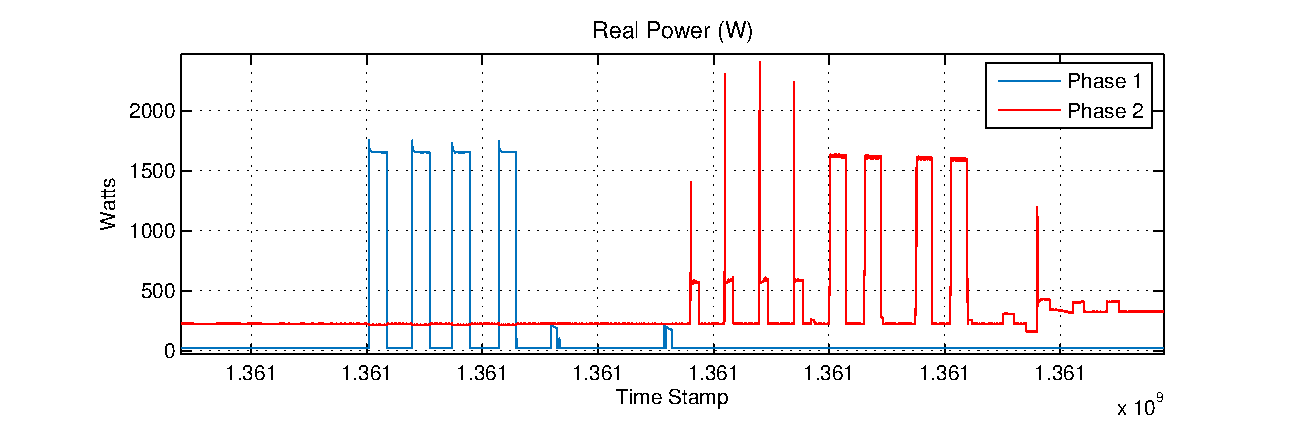
\includegraphics[width=3.5in,height = 1.05in]{fig/exTrain.eps}
		\label{fig:event1ml}}
	\hfil
	\subfloat[Test]{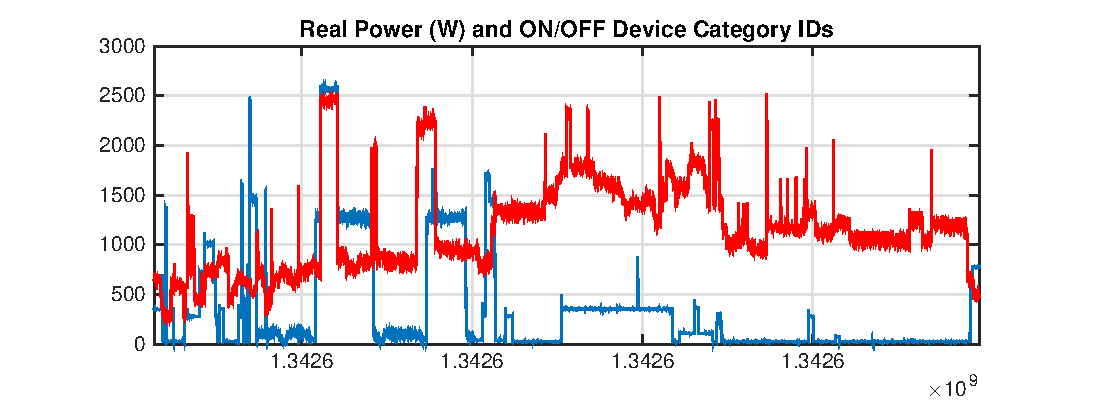
\includegraphics[width=3.5in,height = 1.05in]{fig/exTestH2_1.eps}
		\label{fig:event2ml}}
	%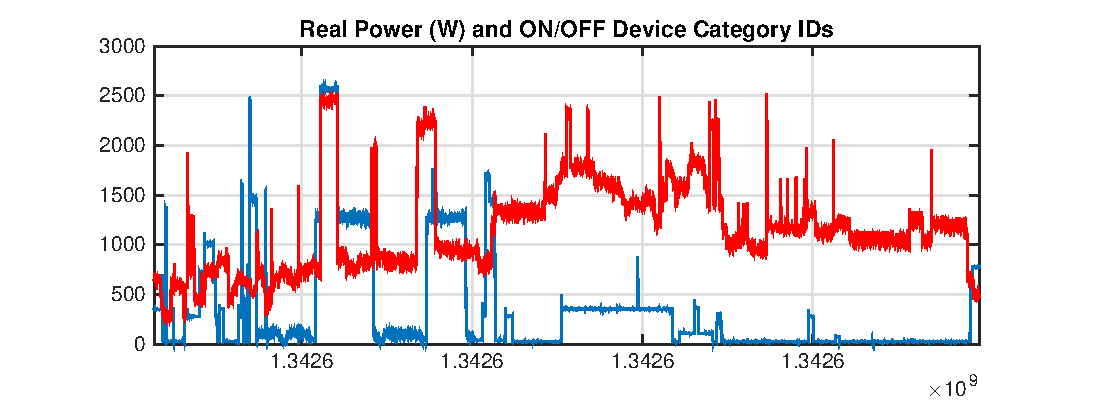
\includegraphics[width=3.5in]{fig/exTestH2_1.eps}
	\caption{Example of (a) training and (b) test data from Home 2.  In each plot, real power consumption measured from a single point is shown for both phases. } 
	\label{fig:traintest}
\end{figure}

Each training set consists of manually generated power consumption data for each appliance in each home.  The training data is a time-serires where only one appliance is switched on at a time, although background noise can be present from untagged appliances. Tagging labels in the training data are also provided, however, these are not always precise enough to correctly identify device turn-on and turn-off times. Correction of tagging labels for training data is therefore needed and is discussed in Section \ref{sec:training}.  Fig.\ref{fig:traintest} shows an example of both training and test data from H2.  The observations recorded in each training and test set cover approximately 24 hours.  

\subsection{Methodology}
Our goal is to develop an interpretable yet effective classification approach.  It can be observed from Fig. \ref{fig:traintest} (b) that the test data is the aggregated load of multiple appliances.  Therefore, at any given time, it is not possible to determine which appliances are operating by using only the level of power consumption.  However, when an appliance is turned on or off, a step change is produced in real and reactive power.  By comparing the average power consumed before and after these transient events, we can calculate averaged power differences, facilitating discrimination among appliances.  For this reason, our methodology focuses on detecting unique turn-on and turn-off signatures in the power differences domain for each appliance.  A flow chart of the proposed methodology is shown in Fig. \ref{fig:flow}.

The first step is to extract transient signature windows for each appliance.  Raw data is converted from the power domain (P and Q) into the power differences domain ($\Delta P_{avg}$ and $\Delta Q_{avg}$) by taking the difference of two moving average windows in P and Q.  After $\Delta P_{avg}$ and $\Delta Q_{avg}$ are calculated, transient signature windows are extracted for each appliance.  Choosing the appropriate window length is a key component to this step and the procedure is explained in detail in Section \ref{sec:training}. 

Once transient signatures are extracted for each appliance in the training data, cross-validation is performed.  This step involves moving  $\Delta P_{avg}(n)$ or $\Delta Q_{avg}(n)$ past the extracted signature window to calculate the root-mean-squared error (RMSE).  Turn-on and turn-off events are detected when the RMSE falls below a specified threshold simultaneously for both real and reactive power differences.  The ability of each signature window to detect other events of the same appliance in the training data is used to determine if the appliance is detectable or not.  If an appliance cannot be detected during cross-validation, it will not be predicted in the test set.  The procedure to determine the correct threshold and separability of each appliance is presented in Section \ref{sec:cv}.  

Finally, for the test set, we use the cross-validated signature windows and threshold values to calculate RMSE and detect appliance turn-on and turn-off events.  This process is discussed in Section \ref{sec:concl}.  

\begin{figure}[!t]
	\centering
	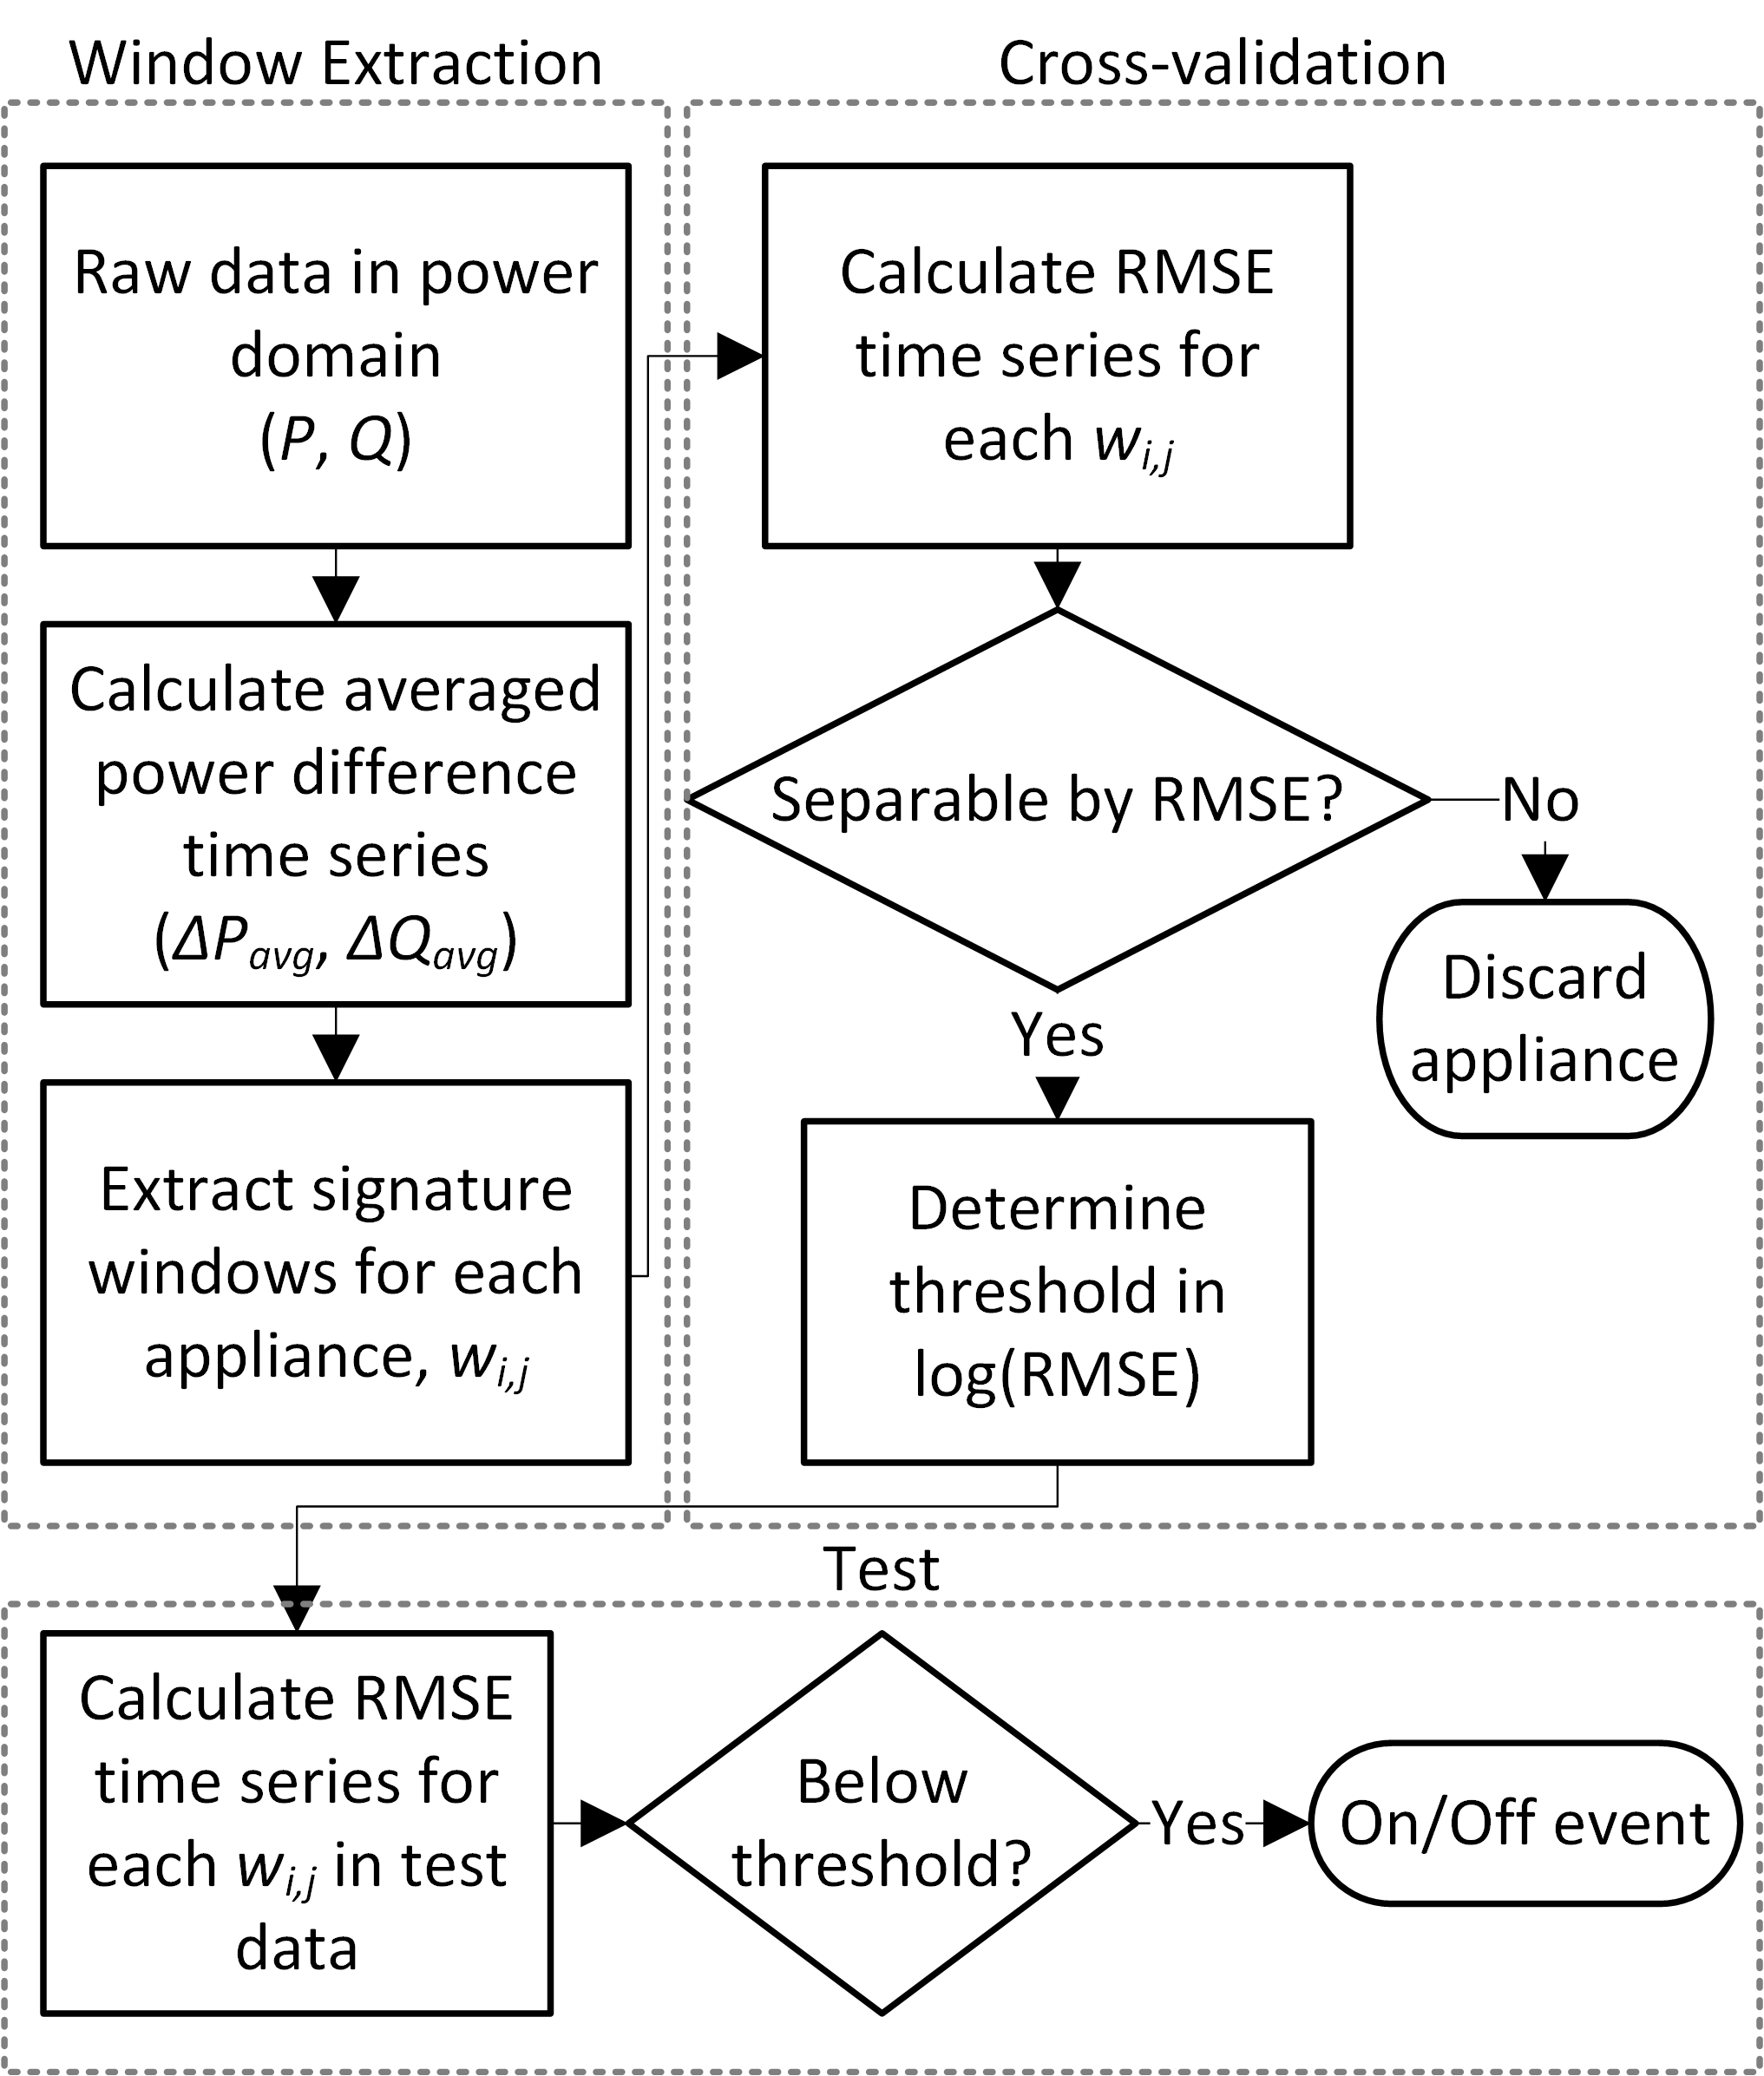
\includegraphics[width=3.3in]{fig/flow.png}
	\caption{Flow chart of proposed methodology.  The procedure is separated into window extraction, cross-validation, and application to test data.}
	\label{fig:flow}
\end{figure}

%
%
%
%\begin{figure}[!t]
%	\centering
%%	\subfloat[]{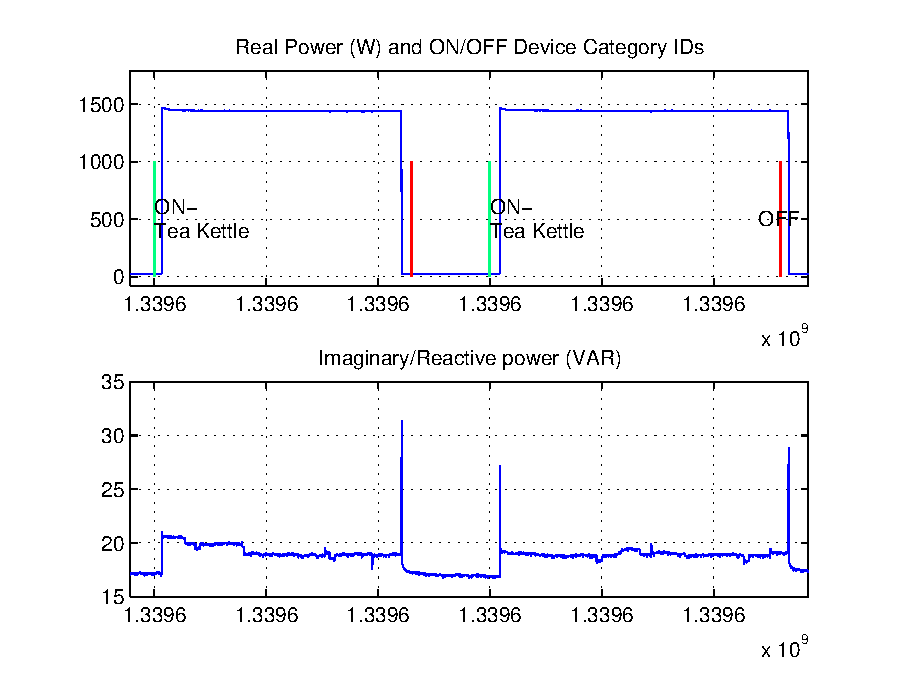
\includegraphics[width=1.7in]{fig/kettle.eps}
%%		\label{fig:event1}}
%	\subfloat[]{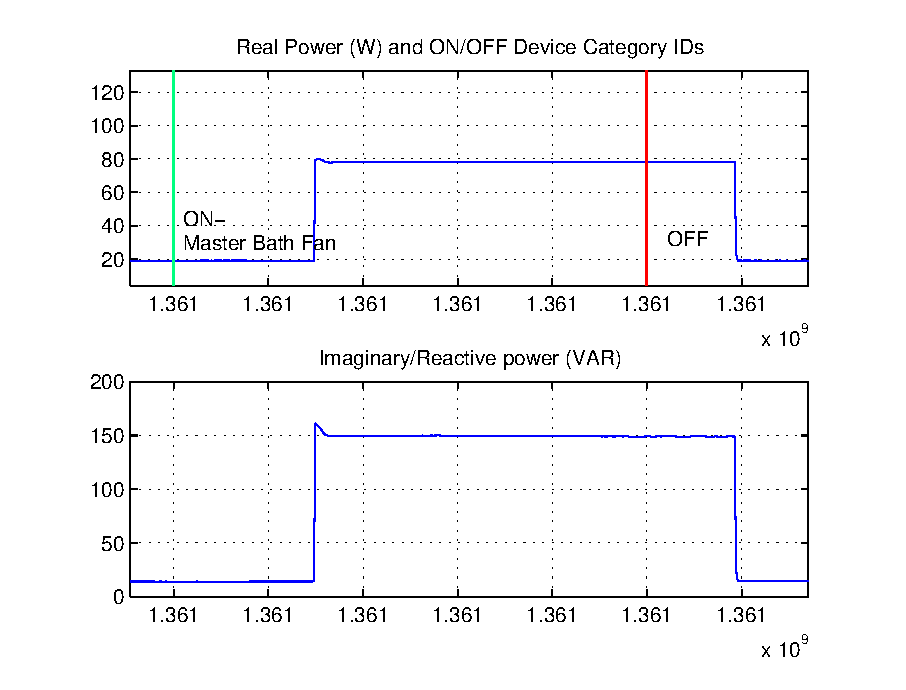
\includegraphics[width=3.5in, height = 1in]{fig/fan.eps}
%		\label{fig:event2}}
%	\hfill
%%	\subfloat[]{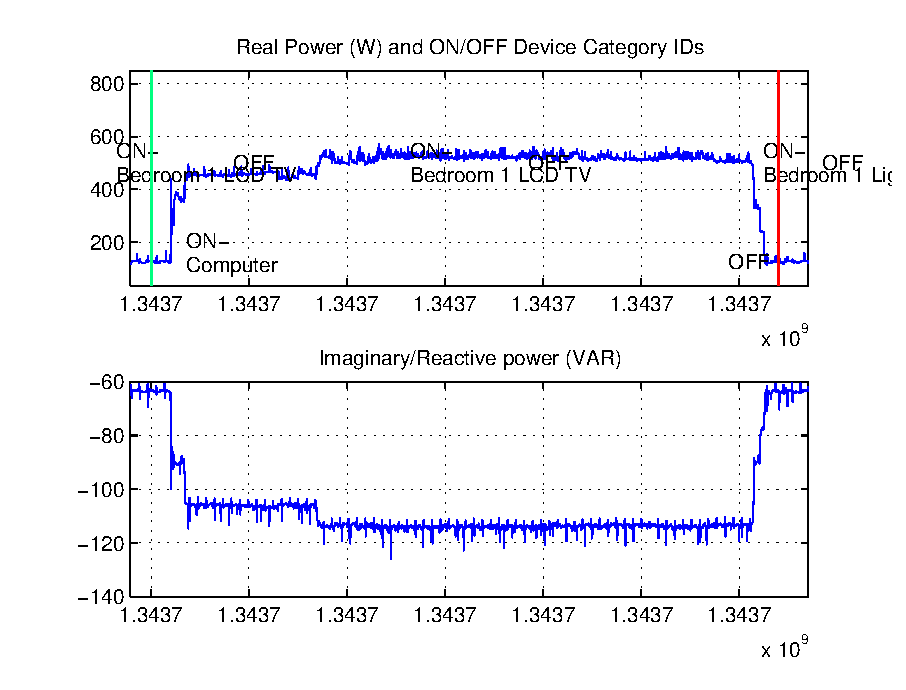
\includegraphics[width=1.7in]{fig/computer1.eps}
%%		\label{fig:event1}}
%	\subfloat[]{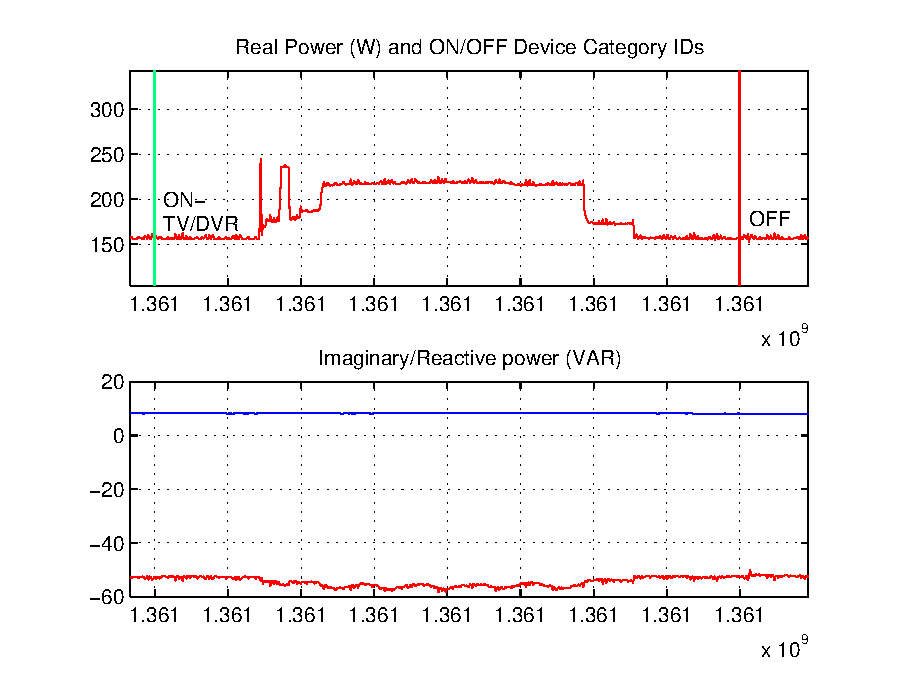
\includegraphics[width=3.5in,height = 1in]{fig/TV.eps}
%		\label{fig:event2}}
%	\hfill
%	\subfloat[]{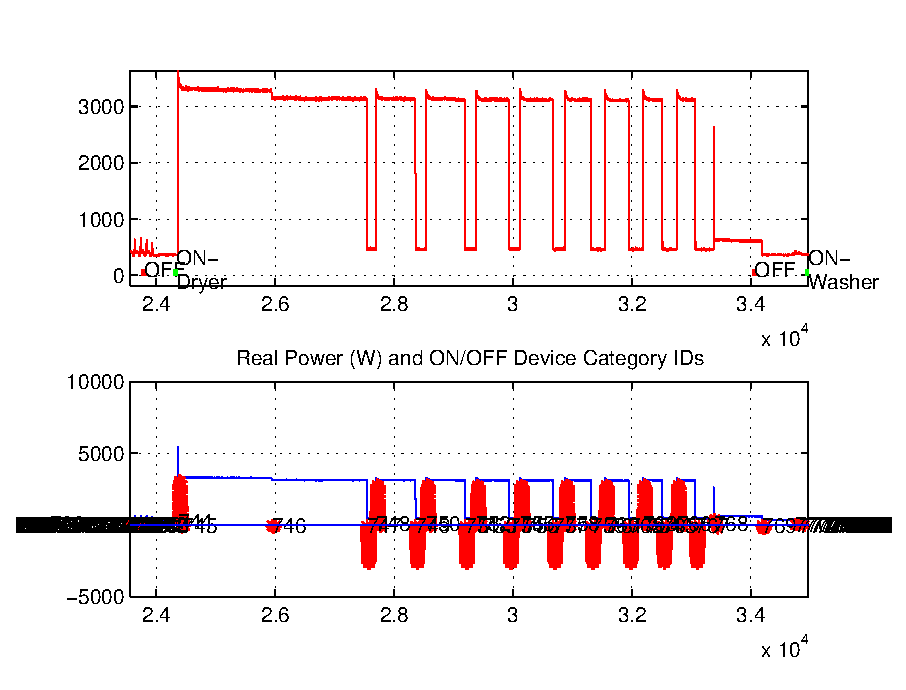
\includegraphics[width=3.5in,height = 1in]{fig/dryer.eps}
%		\label{fig:event1}}
%%	\subfloat[]{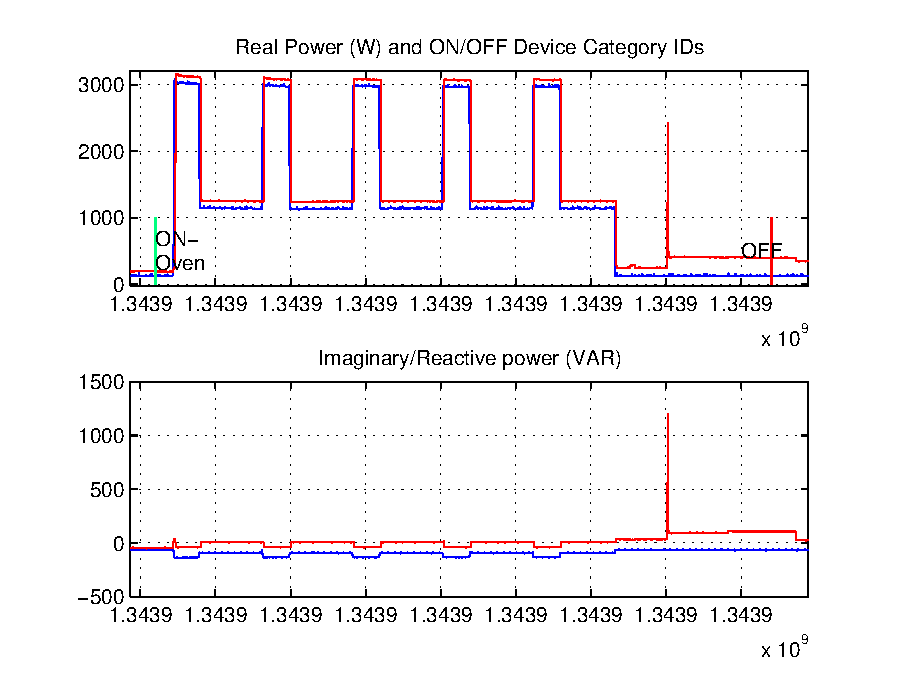
\includegraphics[width=1.7in]{fig/oven.eps}
%%		\label{fig:event2}}
%	\caption{Load Types (a) Tea Kettle, (b) Master Bath Fan, (c) Computer, (d) TV, (e) Dryer, (f) Oven.}
%	\label{fig:exLoads}
%\end{figure}	

\section{Signature Window Extraction}\label{sec:training}
This section describes how transient signature windows are extracted by using averaged real and the reactive power differences.  In particular, a pair of turn-on and turn-off signature windows are trained for every event of each appliance in the training data.  The following sections describe how the signature windows are extracted.  


\subsection{Load Types}
The appliances are first categorized into three load types based on their load shape in P and Q.  The types include rectangular, non-rectangular, and cyclic loads:

\begin{enumerate}
\item{Rectangular loads:} These type of loads consume constant power when operating and their transient period is characterized by a sharp transition from zero to rated power consumption.  Their load shapes are generally rectangular and consist of primarily resistive loads, such as lights, heaters, and kettles.  Some inductive loads, such as small fans, also exhibit this load shape.  A short duration window consisting of the real and the reactive power differences are used to detect these loads.
\newline
\item{Non-rectangular loads:} These type of loads have a longer transient period when turning on and include computers and TVs.  Their transient period is characterized by a stepwise transition from zero to rated power consumption.  Although the power consumed may vary based on how the device is operated, the turn-on signatures can be unique, allowing discrimination against other devices.  These type of loads require a longer window length to capture the unique transient shape.
\newline
\item{Cyclical loads:} - The amount of real or reactive power consumed by these loads change depending on the cycle of their operation.  Dryers, ovens, and washers are included in this category.   However, because they operate on set cycles, there are only a few possible periodic load shapes they can follow.  A modified approach is required to detect these type of loads: identifying a notable recurrent patterns during appliance operation.
\end{enumerate}

%Illustrative examples of these load types are shown in Fig. \ref{fig:exLoads}.  The dryer for example produces several rectangular step changes over the course of its cycle, resulting in misclassifications if not accounted for.  The modified approach for detecting these appliance is discussed below.

\subsection{Averaged Power Differences}
Our approach relies on identifying appliance turn-on and turn-off events by detecting unique transient signatures in real and reactive power consumption. To extract transient signatures for each appliance, the averaged power differences are calculated from two moving average windows.  The averaged differences for real power, $\Delta P_{avg}(n)$, is defined as,
\begin{equation}
\Delta P_{avg}(n) = \frac{1}{N}\sum_{k=0}^{N-1}P(n-k) - \frac{1}{N}\sum_{k=N+D}^{2N+D-1}P(n-k)
\end{equation}
where $N$ is the window size and $D$ is the distance between the two windows.  The averaged differences for reactive power, $\Delta Q_{avg}(n)$, is calculated using the same $N$ and $D$.  It should be noted that if a shorter window size is used, it is easier to distinguish events happening at the same incidence.  However, the detector becomes less robust to noise.

\begin{figure}[!t]
	\centering
	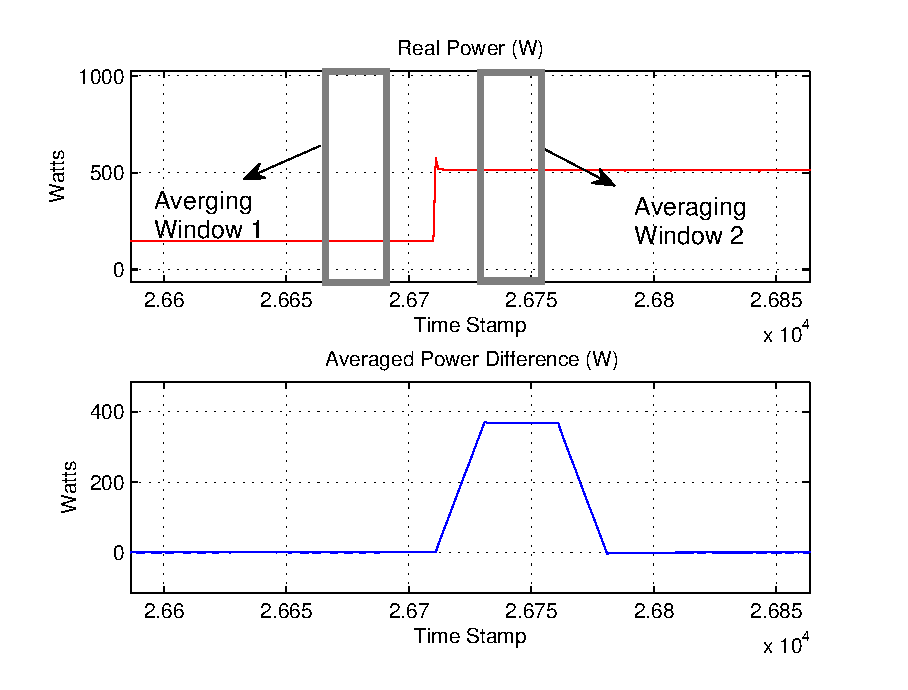
\includegraphics[width=3.5in]{fig/maw.eps}
	\caption{Difference of two moving average windows to detect transient signatures.}
	\label{fig:maw}
\end{figure}

Using the averaged power differences to determine true appliance event indices, tagging labels from the raw data are first corrected.  A threshold in real power differences is then set to indicate whether an event occurred, (i.e., an event occurred if $|\Delta P_{avg}(n)| >$ threshold).  Then the corrected indices are used as the actual event index instead of the tagging info provided in the raw data.  On the top plot of Fig. \ref{fig:tagging}, the tagging labels of the bedroom lights do not align with the actual event incidence.  The bottom plot shows when the first index of the averaged power difference is greater than the threshold; this index is used as the corrected tagging label.  It should be noted that some appliances that consume very small real or reactive power are discarded as they cannot be detected.  For these appliances, using real and reactive power differences will cause false detections in the test data due to the effects of the noise.  Additional features must be considered to detect such appliances.

\begin{figure}[!t]
	\centering
	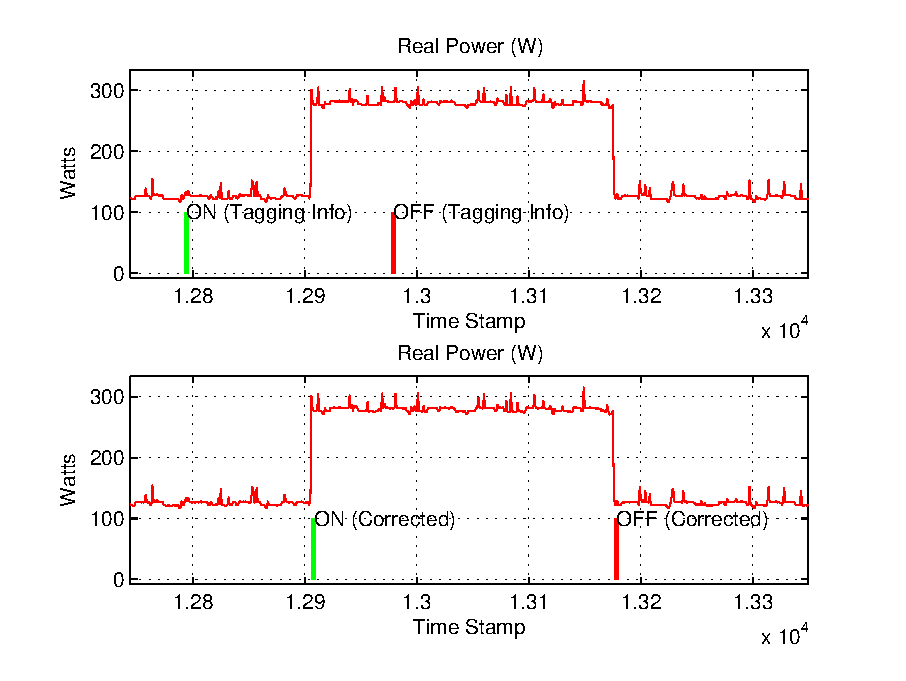
\includegraphics[width=3.5in]{fig/tagginginfo.eps}
	\caption{Provided tagging labels are corrected in the power differences domain.}
	\label{fig:tagging}
\end{figure}
	

\subsection{Window Extraction}
After taking the power differences, the next step is to extract the signatures for turn-on  and turn-off events. The windows are extracted using the corrected tagging labels.  For rectangular load shapes, the transient signature window is extracted from the start of the turn-on event until the load reaches steady-state power consumption.  If an appliance has longer transient characteristics (non-rectangular load shapes), longer window sizes are used to capture the entire unique transient period.  For example, consider the dining room light and the laptop charger profile shown in Fig. \ref{fig:windowlength}.  Both the appliances consume about 38 W at event incidence.  However, the laptop charger then spends additional 38 Watts to fully turn on.  Therefore, a longer window length is needed to detect the laptop charger than the dining room lights. 

\begin{figure}[!t]
	\centering
	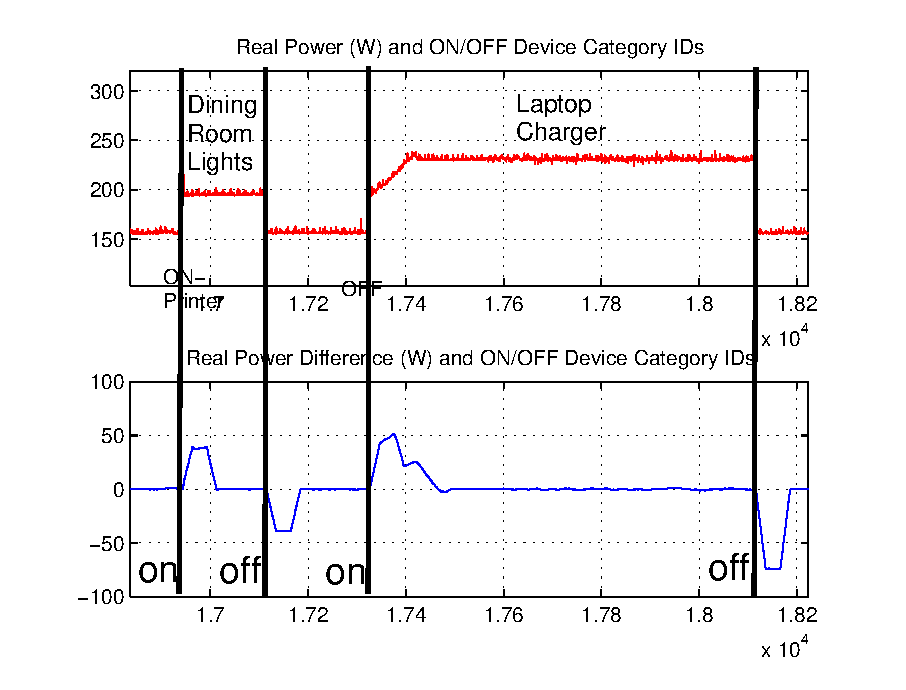
\includegraphics[width=3.5in]{fig/windowlength.eps}
	\caption{Example of how choosing the appropriate window length can affect classification.}
	\label{fig:windowlength}
\end{figure}

Cyclical loads exhibit unique characteristics that are different from the rectangular and the non-rectangular loads.  These types of appliances are difficult to be detected by using turn-on and turn-off signature windows because each step change in power consumption during the cycle can be mistaken for other appliances..  Therefore, for cyclical loads only, a window is trained to capture unique signatures during their operation.  Consider the dryer in Home 2 as shown in Fig. \ref{fig:dryerH2}.  The load shape of the dryer has multiple sharp peaks during its operation.  Therefore, a single window can be trained to detect these sharp peaks.  In this case, the following rule can be made:  "While the recurrent pattern window is detecting an event, the appliance is operating."  

Outlier detection is also held during this stage.  Consider the four on/off events of a computer as shown in Fig. \ref{fig:outlier}.  It can be seen that when event two occurred, some background noise affected the turn-on signature of the computer.  In this case, the second event is regarded as an outlier and is not used in training the windows.  When the window extraction procedure is complete transient signature windows are defined for all detectable events.  

\begin{figure}[!t]
	\centering
	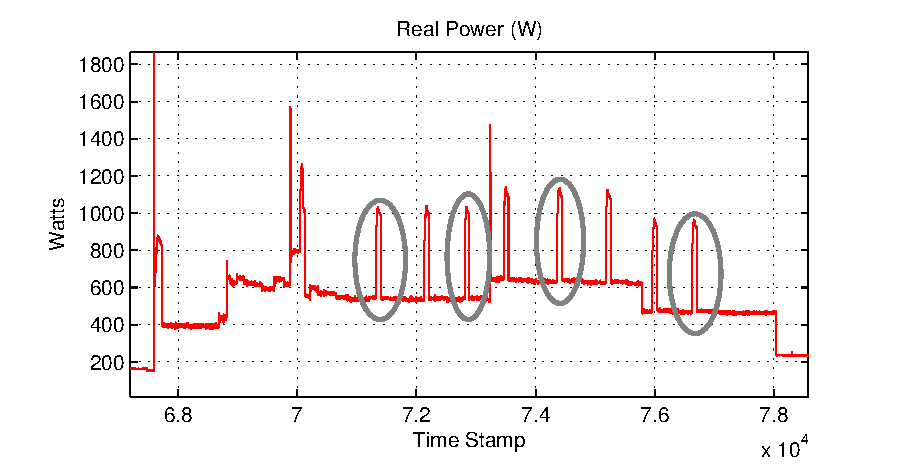
\includegraphics[width=3.5in]{fig/dryerH2.eps}
	\caption{Unique Characteristics of Dryers in Home 2.}
	\label{fig:dryerH2}
\end{figure}
	
\begin{figure}[!t]
	\centering
	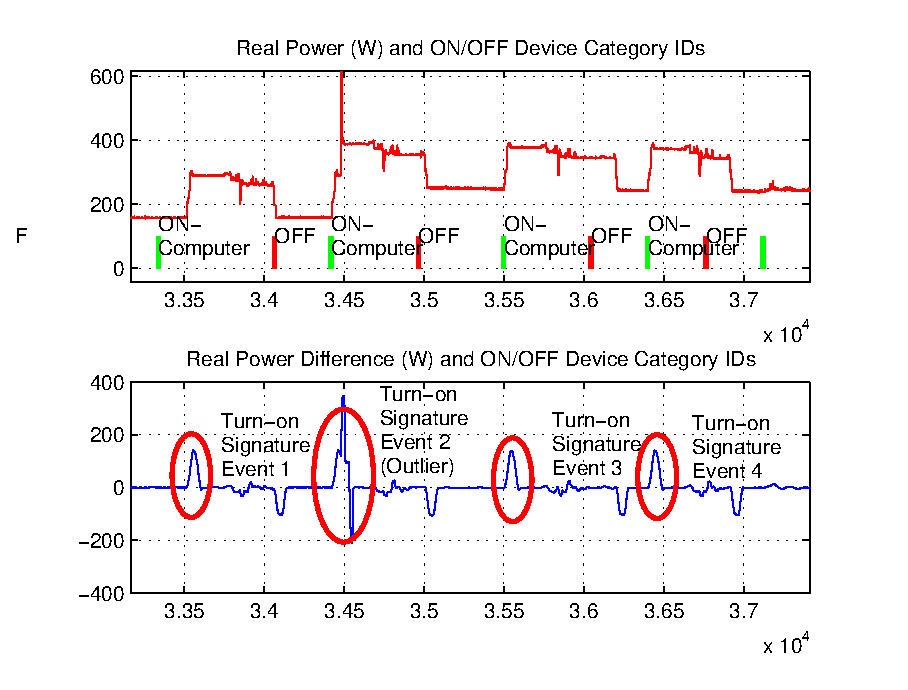
\includegraphics[width=3.5in]{fig/outlier.eps}
	\caption{Computer turn-on event outlier shown in the 2nd event.}
	\label{fig:outlier}
\end{figure}


% An example of a floating figure using the graphicx package.
% Note that \label must occur AFTER (or within) \caption.
% For figures, \caption should occur after the \includegraphics.
% Note that IEEEtran v1.7 and later has special internal code that
% is designed to preserve the operation of \label within \caption
% even when the captionsoff option is in effect. However, because
% of issues like this, it may be the safest practice to put all your
% \label just after \caption rather than within \caption{}.
%
% Reminder: the "draftcls" or "draftclsnofoot", not "draft", class
% option should be used if it is desired that the figures are to be
% displayed while in draft mode.
%
%\begin{figure}[!t]
%\centering
%\includegraphics[width=2.5in]{myfigure}
% where an .eps filename suffix will be assumed under latex, 
% and a .pdf suffix will be assumed for pdflatex; or what has been declared
% via \DeclareGraphicsExtensions.
%\caption{Simulation Results.}
%\label{fig_sim}
%\end{figure}

% Note that IEEE typically puts floats only at the top, even when this
% results in a large percentage of a column being occupied by floats.


% An example of a double column floating figure using two subfigures.
% (The subfig.sty package must be loaded for this to work.)
% The subfigure \label commands are set within each subfloat command,
% and the \label for the overall figure must come after \caption.
% \hfil is used as a separator to get equal spacing.
% Watch out that the combined width of all the subfigures on a 
% line do not exceed the text width or a line break will occur.
%
%\begin{figure*}[!t]
%\centering
%\subfloat[Case I]{\includegraphics[width=2.5in]{box}%
%\label{fig_first_case}}
%\hfil
%\subfloat[Case II]{\includegraphics[width=2.5in]{box}%
%\label{fig_second_case}}
%\caption{Simulation results.}
%\label{fig_sim}
%\end{figure*}
%
% Note that often IEEE papers with subfigures do not employ subfigure
% captions (using the optional argument to \subfloat[]), but instead will
% reference/describe all of them (a), (b), etc., within the main caption.


% An example of a floating table. Note that, for IEEE style tables, the 
% \caption command should come BEFORE the table. Table text will default to
% \footnotesize as IEEE normally uses this smaller font for tables.
% The \label must come after \caption as always.
%
%\begin{table}[!t]
%% increase table row spacing, adjust to taste
%\renewcommand{\arraystretch}{1.3}
% if using array.sty, it might be a good idea to tweak the value of
% \extrarowheight as needed to properly center the text within the cells
%\caption{An Example of a Table}
%\label{table_example}
%\centering
%% Some packages, such as MDW tools, offer better commands for making tables
%% than the plain LaTeX2e tabular which is used here.
%\begin{tabular}{|c||c|}
%\hline
%One & Two\\
%\hline
%Three & Four\\
%\hline
%\end{tabular}
%\end{table}


% Note that IEEE does not put floats in the very first column - or typically
% anywhere on the first page for that matter. Also, in-text middle ("here")
% positioning is not used. Most IEEE journals/conferences use top floats
% exclusively. Note that, LaTeX2e, unlike IEEE journals/conferences, places
% footnotes above bottom floats. This can be corrected via the \fnbelowfloat
% command of the stfloats package.



\section{Cross-Validation}\label{sec:cv}
In this section, we present the procedure for cross-validating the signature windows trained in Section \ref{sec:training} in the training set.  The objective of cross-validating the signature windows of each appliance is to verify the ability to detect other events of the same appliance in the training data.  The root-mean-squared error (RMSE) is chosen as the metric to determine how well the signature window matches with the measured signal.  The equations for calculating RMSE are shown in (\ref{eq:RMSE-P}) and (\ref{eq:RMSE-Q}).
\begin{align}
\label{eq:RMSE-P}
\text{RMSE}_{\text{P}}(n) &= \sqrt{\frac{1}{N}\sum\limits_{k=1}^{N}(w_{i,j}(k) - \Delta P_{avg}(n+k))^2}\\
\label{eq:RMSE-Q}
\text{RMSE}_{\text{Q}}(n) &= \sqrt{\frac{1}{N}\sum\limits_{k=1}^{N}(w_{i,j}(k) - \Delta Q_{avg}(n+k))^2}
\end{align}
where $w_{i,j}$ is the transient signature window for $j$-th turn-on or turn-off event for appliance number $i$.  For each $w_{i,j}$ the procedure for cross-validation is presented in Fig \ref{fig:flow}.

%\begin{algorithm}
%	\caption{Cross-validation Algorithm}\label{euclid}
%	\begin{algorithmic}[1]
%		\For{every time instant $n_0$}	
%
%		\State Calculate $\text{RMSE}_{\text{P}}(n_0)$ and $\text{RMSE}_{\text{Q}}(n_0)$
%		\If{$\text{RMSE}_{\text{P}}(n_0)<\theta_P$ and $\text{RMSE}_{\text{Q}}(n_0)<\theta_Q$ } 
%		determine if threshhold (theta) exists for which log(RMSE)<1.3*theta is able to detect 100 \% of appliances i in the training set and none of the other  N-1 appliances in the training set
%		
%		\State Event is detected at time instant $n_0$
%		\EndIf
%		%		\EndFor
%		\EndFor
%	\end{algorithmic}
%\end{algorithm}
%
%This step involves moving  $\Delta P_{avg}(n)$ or $\Delta Q_{avg}(n)$ past the extracted signature window to calculate the root-mean-squared error (RMSE).  
%apply signature window w(n)i,j
% (that's why 1.3*theta)
%need to determine P and Q thresholds simultaneously
%Turn-on and turn-off events are detected when the RMSE falls below a specified threshold simultaneously for both real and reactive power differences.    If an appliance cannot be detected during cross-validation, it will not be predicted in the test set.  

Both $\text{RMSE}_{\text{P}}$ and $\text{RMSE}_{\text{Q}}$ will simultaneously reach a minimum when the associated appliance turns on or off in the averaged power differences domain. However, other appliances switching on and off can cause $\text{RMSE}_{\text{P}}$ and $\text{RMSE}_{\text{Q}}$ value to rise, fall, or stay the same.  It is possible that both the RMSE values drop when the window is detecting different appliance.  This happens when the signature windows of the two appliances have a very similar shape and amplitude.  To prevent this scenario, RMSE thresholds ($\theta_P$ and $\theta_Q$) are set to prevent other appliances from being detected.  If such thresholds ($\theta_P$ and $\theta_Q$) can not be set, the window is discarded.  Figure \ref{fig:bread} shows an example of this procedure. The window successfully detects the breadmaker turning-on with all the other events being rejected. 

\begin{figure}[!t]
	\centering
	\includegraphics[width=3.5in]{fig/cv_bread.eps}
	\caption{Cross-validation of appliance "breadmaker" for two events in the training data.}
	\label{fig:bread}
\end{figure}

\begin{table}[!t]
	\renewcommand{\arraystretch}{1.3}
	\caption{Number of Appliances Validated and Discarded for Each Home}\label{classes}
	\label{table:cv}
	\centering
	\begin{tabular}{c||c||c||c}
		\hline 
		\textbf{Home No.} & \textbf{Total Appliances} &\textbf{Discarded} &\textbf{No. Validated (\%)}\tabularnewline
		\hline 
		\hline 
		H1 & 38 & 11 & 27 (71.1\%)\tabularnewline
		\hline 
		H2 & 37 & 6 & 31 (83.8\%)\tabularnewline
		\hline 
		H3 & 37 & 5 & 32 (86.5\%)\tabularnewline
		\hline 
		H4 & 36 & 9 & 27 (75.0\%)\tabularnewline
		\hline 
	\end{tabular}
\end{table}


\section{Test Data}\label{sec:test}
We then apply our algorithm on the provided test data and identify appliance on and off intervals.  The detections are made from the signature windows we extracted from the training set with the threshold values acquired from cross-validation.  The algorithm is shown below and is applied for every extracted signature window $w_{i,j}(n)$.

\begin{algorithm}
	\caption{Event Detection Algorithm}\label{euclid}
	\begin{algorithmic}[1]
	\For{every time instant $n_0$}	
%		\ForAll{$w_{i,j}$}
			\State Calculate $\text{RMSE}_{\text{P}}(n_0)$ and $\text{RMSE}_{\text{Q}}(n_0)$
			\If{$\text{RMSE}_{\text{P}}(n_0)<\theta_P$ and $\text{RMSE}_{\text{Q}}(n_0)<\theta_Q$ } 
			\State Event is detected at time instant $n_0$
			\EndIf
%		\EndFor
	\EndFor
	\end{algorithmic}
\end{algorithm}

Although the competition has closed, we are ableo to submit our predictions and see its rank compared to past submissions. Our best submission would have placed 7th overall.  However, the strategy for the test data is modified to achieve the best score.  Because scoring is based on average Hamming distance, thresholds are adjusted so that only the most likely predictions, i.e., low RMSE values are predicted.  

\section{Conclusion}\label{sec:concl}
From our cross-validation and test data submission results, the proposed strategy can be a simple yet effective method for household energy usage disaggregation. One of the advantages of this approach is that it is more interpretable because it follows an intuitive approach for detecting appliance on and off events.  With the proposed approach, misclassifications can be traced back to the signature window length or detection thresholds.  This is particularly true when compared to methods utilizing ``black box" predictive models such as artificial neural networks.  Furthermore, the proposed approach as the ability for real time processing. Because calculations are implemented as sliding windows, data can be streamed into the algorithm. Additionally, this method only utilized a subset of the entire dataset, needing only P and Q measurements.  High frequency features could have been added to help classify smaller appliances that were discarded during cross-validation.  However, one of the primary drawbacks is that manual identification of appropriate window lengths is requried during training.  Future work would consider automation of appropriate window lengths.



%-constant power - static: can be difficult if rated power is similar between two appliances, same for below.
%- resistive (lights, heaters, kettle) - P domain and rectangular mainly, can be separated in P domain only if turn on/off signature is unique or if rated power is not similar to others
%- resistive + reactive (rotating like fans) - Q is a feature to help classify; if P is not unique, but Q is, greatly increases classification
%-dynamic
%	- cyclical (washer dryer) - require rules, ie. recurrent pattern detection
%	also high freqency domain for hard to identify appliances.  you can get 7th w/ just P/Q alone.   
	









% conference papers do not normally have an appendix


% use section* for acknowledgement
%\section*{Acknowledgment}
%
%
%The authors would like to thank...





% trigger a \newpage just before the given reference
% number - used to balance the columns on the last page
% adjust value as needed - may need to be readjusted if
% the document is modified later
%\IEEEtriggeratref{8}
% The "triggered" command can be changed if desired:
%\IEEEtriggercmd{\enlargethispage{-5in}}

% references section

% can use a bibliography generated by BibTeX as a .bbl file
% BibTeX documentation can be easily obtained at:
% http://www.ctan.org/tex-archive/biblio/bibtex/contrib/doc/
% The IEEEtran BibTeX style support page is at:
% http://www.michaelshell.org/tex/ieeetran/bibtex/
%\bibliographystyle{IEEEtran}
% argument is your BibTeX string definitions and bibliography database(s)
%\bibliography{IEEEabrv,../bib/paper}
%
% <OR> manually copy in the resultant .bbl file
% set second argument of \begin to the number of references
% (used to reserve space for the reference number labels box)

%\begin{thebibliography}{1}
%
%\bibitem{IEEEhowto:kopka}
%H.~Kopka and P.~W. Daly, \emph{A Guide to \LaTeX}, 3rd~ed.\hskip 1em plus
%  0.5em minus 0.4em\relax Harlow, England: Addison-Wesley, 1999.
%
%\end{thebibliography}

%\begin{thebibliography}{1}
%
%\end{thebibliography}

\bibliography{Bib}
\bibliographystyle{ieeetr}



% that's all folks
\end{document}


